\chapter{Code Changes in the Execution Manager}
\label{chapter:KiemChanges}
Although the project attempts to realize most of the objectives without
changing the Execution Manager itself minimal adaptations were necessary.
This mostly involves adding new methods to the \ac{API} in order to
gain access to previously hidden properties.

Also some changes had to be performed where properties were loaded from hard-coded 
default values. These were refined and will now only be used if the \ac{KIEMConfig} 
plug-in is not registered to supply previously saved properties.

However all changes that were made to the \ac{KIEM} plug-in were merely additions
and won't break any plug-ins relying on the old implementation.

\section{Schema Files and Interfaces}
\index{Extension point}
In order to provide additional functionality for other plug-ins we choose the extension
point mechanism described in Section \ref{section:TechExtension}. This is done
is order to retain the old functionality of the plug-in while on the other hand giving
options to ask extending plug-ins for their contributions. 

The extension points are described in more details in the next sections. They consist
of a schema file for defining the extension point and an interface that contains the 
methods that extending components have to supply.

\subsection{Toolbar Contribution Provider}
\label{section:ToolbarContributionProvider}
\index{Toolbar Contribution Provider}
The purpose of the tool bar contribution provider is to allow other plug-ins to put
items onto the tool bar of the Execution Manager. 
There are two reasons for using the extension point mechanism
rather than making the tool bar available and have other plug-ins put their
contributions directly on it:
\begin{enumerate}
 \item At the moment the tool bar and all contributions are created dynamically. Switching
the entire native tool bar of the Execution Manager to adding the actions to the tool bar
through a predefined Eclipse extension point would require major code changes and
have major drawbacks.
 \item A programmatic approach gives control over the contributions to the Execution Manager.
This means that the order of the native Execution Manager buttons is always the same and in the
same place. It also means that the Execution Manager can choose to ignore contributions if the
tool bar gets too crowded.
\end{enumerate}
\begin{figure}[IToolbarContributor]
  \centering
  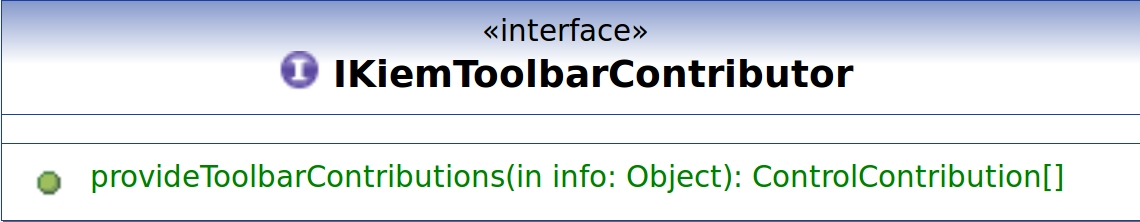
\includegraphics[scale=.3]{IKiemToolbarContributor.jpg}
  \caption[The interface for Tool bar Contribution Providers]%
  {The interface for Tool bar Contribution Providers\protect}
  \label{fig:IToolbarContributor}
\end{figure}

The schema file for components that want to add contributions to the tool bar is quite simple.
It only requires them to implement the interface shown in figure \ref{fig:IToolbarContributor}.
The implementing class provides an array with all ControlContributions they want to add to the tool bar.
A ControlContribution for a tool bar can be almost any widget like Labels, Buttons, ComboBoxes, ....

When the Execution Manager starts to build the views tool bar it will perform the following steps:
\begin{enumerate}
 \item The contributors will be asked for the list of controls that they want to contribute.
 \item That list will be added to the Execution Manager's tool bar.
 \item After that the Execution Manager will add its own controls to the tool bar.
\end{enumerate}
This order causes the tool bar to have the native elements always in the same order.
The contributed elements will be added from left to right in the order that they occur in the array. However there
is no guarantee on the order in which the extending plug-ins are asked.
Figure \ref{fig:ToolbarWithContributions} shows the Execution Manager tool bar with the two combo boxes belonging to \ac{KIEMConfig}
contributed through the extension point. Figure \ref{fig:ToolbarWithoutContributions} shows the same tool bar without
the contributions.
\begin{figure}[ToolbarWithContributions]
  \centering
  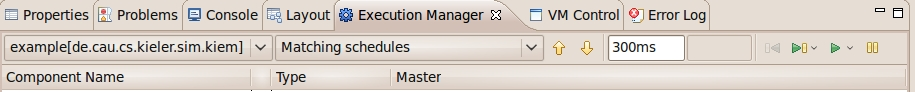
\includegraphics[scale=.4]{ToolbarWithContributions.jpg}
  \caption[The Execution Managers Tool bar with two contributed ComboBoxes]%
  {The Execution Managers Tool bar with two contributed ComboBoxes\protect}
  \label{fig:ToolbarWithContributions}
\end{figure}
\begin{figure}[ToolbarWithoutContributions]
  \centering
  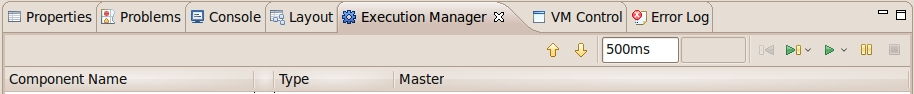
\includegraphics[scale=.4]{ToolbarWithoutContributions.jpg}
  \caption[The Execution Managers Tool bar without contributions]%
  {The Execution Managers Tool bar without contributions\protect}
  \label{fig:ToolbarWithoutContributions}
\end{figure}

\subsection{Configuration provider}
\label{section:ConfigurationProvider}
\index{Configuration Provider}
The purpose of the configuration provider is to allow internal attributes of the
Execution Manager to be stored in another plug in. 

This is achieved by another extension point to allow any plug-in to listen to changes
in the Execution Manager's attributes. It also means that there may be multiple
plug-ins that provide values for properties and not all plug-ins may have the value for
a property needed by the Execution Manager. Through the plug-in mechanism the \ac{KIEM}
can ask all providers for values and choose the one he would like to use.

\begin{figure}[Configuration Provider Interface]
  \centering
  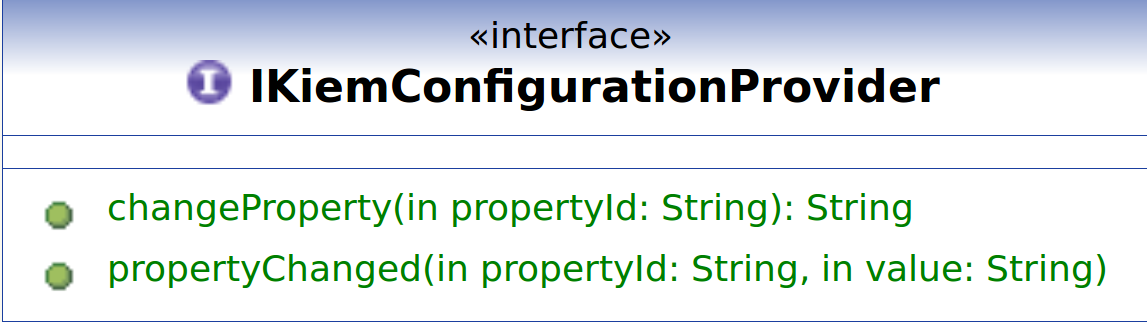
\includegraphics[scale=0.3]{IKiemConfigurationProvider.png}
  \caption[The Interface of the Configuration Provider]%
  {The Interface of the Configuration Provider\protect}
  \label{fig:UMLConfigurationProvider}
\end{figure}

The two methods from the interface shown in Figure \ref{fig:UMLConfigurationProvider} work
in the following way:

\subsection{Event Listener}
\label{section:EventListener}
The main purpose of the Event Manager is to inform DataComponents of events
happening in the Execution Manager during execution. This behavior has been modified to include 
events that occur while the execution is not running. This modification lead to the 
creation of another extension point in order to allow other plug-ins to be notified
on any of these events as well. The classes implementing the interface 
(see Figure \ref{fig:UMLEventListener}) required by this extension point will be notified
on any event that happens inside the Execution Manager.

\begin{figure}[Event Listener Interface]
  \centering
  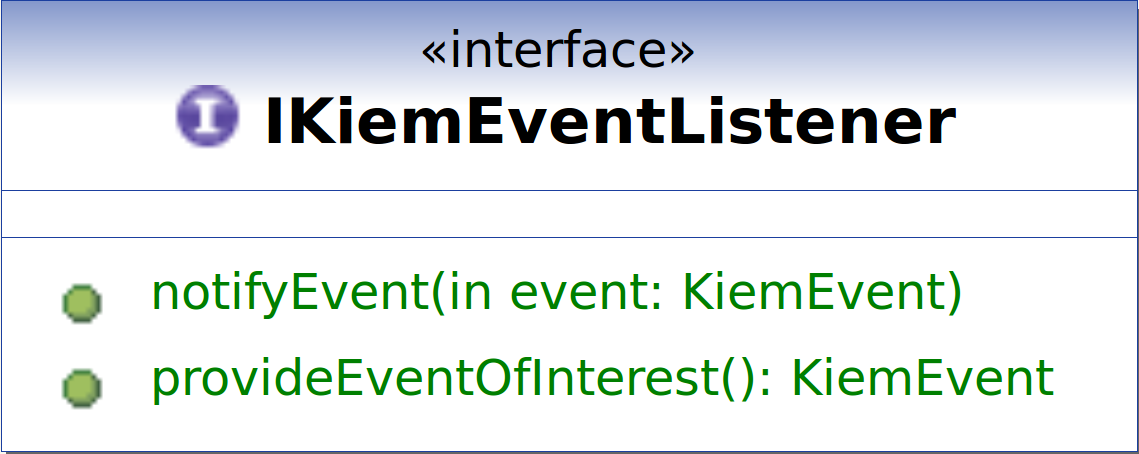
\includegraphics[scale=0.3]{IKiemEventListener.png}
  \caption[The Interface of the Event Listener]%
  {The Interface of the Event Listener\protect}
  \label{fig:UMLEventListener}
\end{figure}

The semantics of the methods will be explained in detail in the following two subsections.

\subsubsection*{provideEventOfInterest()}
This method is directly derived from the method with the same name in the AbstractDataComponent class
of the \ac{KIEM} plug-in. It is called by the EventManager to determine which events the implementing
class is interested in. This is done to improve efficiency and not flooding components with events
they are not interested in.

Based on the response, the EventManager puts the component into lists along with the DataComponentWrappers
already inside.
\subsubsection*{notifyEvent(KiemEvent event)}
This method is called by the EventManager when something happens inside the Execution Manager that the implementing
classes might be interested in.


\section{KIEMPlugin.java}
\label{section:ConfChangesKiemPlugin}
The main Activator class contains almost the entire \ac{API} of the \ac{KIEM}.
Therefore any additions to that has to performed in this class which means that
most of the adjustments were made here.

\subsection{Listener}
The following methods were added to communicate with the plug-ins registered through
the ConfigurationProvider extension point (see Section \ref{section:ConfigurationProvider}).
\begin{description}
 \item {notifyConfigurationProviders(String propertyId, String value)} : This method can be called by any class
inside the Execution Manager itself. It should be called when the user changes a property through any of
the elements on the \ac{GUI}. The method will then inform all listeners that the property identified by the
given identifier was changed to the new value.
 \item {String getPropertyValueFromProviders(String propertyId)} : This method allows the Execution Manager to
retrieve a previously saved value. The \ac{KIEM} will ask all plug-ins registered on the extension point if they
can provide a value for the given identifier. Plug-ins that can't provide the value will indicate this by throwing
an Exception. The \ac{KIEM} will then take the first value he receives without getting an Exception and assign it
to the internal property.
 \item {Integer getIntegerValueFromProviders(final String propertyId)} : This method is a convenience method for
the one described above. It will try to parse an integer from the retrieved String and return it or return null
if no integer could be parsed.
\end{description}

\subsection{Getters and Setters}
An example for the use of the methods described in the last section can be found in the Getters and Setters for
the different properties in the Execution Manager (for an example see Figure \ref{fig:getterAndSetter}). 
These were changed in order to use the new methods but are
still able to fall back on hard-coded default values if no configuration plug-in is registered.

\lstset{
  language=Java,
  frame=shadowbox, 
  rulesepcolor=\color{blue},
  caption=The modified Getter and Setter for the step duration,
  label=fig:getterAndSetter,
}
\begin{lstlisting}
public int getAimedStepDuration() {
   int result = this.aimedStepDuration;
   Integer value = getIntegerValueFromProviders(AIMED_STEP_DURATION_ID);
   if (value != null) {
      result = value;
   }
   return result;
}

public void setAimedStepDuration(final int aimedStepDurationi) {
   this.aimedStepDuration = aimedStepDurationi;
   // if executing, also update current delay
   if (execution != null) {
      this.execution.setAimedStepDuration(aimedStepDuration);
   }
   this.getKIEMViewInstance().updateViewAsync();
   notifyConfigurationProviders(AIMED_STEP_DURATION_ID, aimedStepDurationi + "");
}
\end{lstlisting}


\subsection{Open File}
The method that takes care of loading an execution file was split. This was done to allow
other plug-ins to pass an IPath object directly to the method and perform a load of that file without
having to go through the \ac{UI}. This method was also shifted around a little in order to detect
missing execution files before the load enters the UIThread. This was necessary to make is possible for
the callers of the method to catch the resulting exception.
The method also had to be modified in order to be able to take files that are not inside the workspace
but were added through an extension point. The changed part of the openFile method is shown in 
Listing \ref{fig:openFileMethod}.
The last change to that method concerns the event listener. When the user opens a file through the
Eclipse workspace without using the \ac{KIEMConfig} plug-in the plug-in still has to be informed.
This happens through the use of the Event Manager that notifies all listeners upon the successful
completion of the loading operation.

\lstset{
  language=Java,
  frame=shadowbox, 
  rulesepcolor=\color{blue},
  caption=The head of the openFile method,
  label=fig:openFileMethod,
}
\begin{lstlisting}
public void openFile(final IPath executionFile, final boolean readOnly) 
   throws IOException {
   String fileString = executionFile.toOSString();
   final InputStream inputStream;
   
   if (fileString.startsWith("bundleentry:/")) {
      String urlPath = fileString.replaceFirst
         ("bundleentry:/", "bundleentry://");
      URL pathUrl = new URL(urlPath);
      inputStream = pathUrl.openStream();
   } else {
      URI fileURI = URI.createPlatformResourceURI(fileString, true);
      // resolve relative workspace paths
      URIConverter uriConverter = new ExtensibleURIConverterImpl();
      inputStream = uriConverter.createInputStream(fileURI);
   }

   Display.getDefault().syncExec(new Runnable() {
   ...
\end{lstlisting}

\section{KIEMView}
\label{section:ConfChangesKiemView}
The changes described in Section \ref{section:ConfChangesKiemPlugin} were mostly concerned with the
configuration management and loading of new execution files. This section will mostly deal with the changes
that were necessary to enable the adding of new items to the tool bar.

\begin{itemize}
 \item changes to tool bar creation
 \item provide means to set view as dirty when changes happen
 \item refresh method to reload values, not needed before because no change except by user
\end{itemize}